\chapter{Background \& Objectives}

The purpose of this project is to establish whether hybrid mobile applications are a feasible alternative to native development. This will involve exploring, examining and developing apps in a hybrid manner. For this project a music social media app will be developed. The app will have various features e.g. looking up events which take place in  venues. A hybrid mobile application framework will be selected which will form the front end of this project. The back end of this project which will be in PHP.

\section{Background}
There are three different types of mobile applications: a native app, a web app and a hybrid app \cite{BAB} \cite{IIA} \cite{PTA}. A native app is an app which is developed in a platform specific language and is usually downloaded from a device's app store e.g. Google Play Store for Android and the App Store for iOS devices. As  native apps are developed in a platform specific language e.g Android apps are developed in Java \cite{AD} and iOS apps are developed in Swift (formerly Objective C) \cite{ID} this means that  code has to be written in multiple languages to develop the app for different platforms. Native apps allow for platform Application Programming Inteface (APIs) to be used and therefore the developer has access to resources such as the device's camera or contact book \cite{MAC} \cite{MF}.

Web apps are essentially just web pages which are mobile responsive and therefore display well on mobile devices. They are accessed via a device's browser where the user either inputs the uniform resource locator (url) or clicks a link which takes them to the web app. Web apps do not (easily) have access to the platforms' API therefore it is very challenging for a developer to use native resources such as a device's camera \cite{MAC} \cite{BAB} .

Hybrid apps are apps which are written in web technologies (usually HTML5, CSS and JS.) They are usually downloaded through an app store and a piece of middleware enables hybrid apps to have access to native APIs, allowing hybrid apps to access resources such as a device's camera. Unlike native apps, hybrid apps only require one code base for multiple platforms\cite{MAC} \cite{SF}.

\section{Analysis}
It is important to consider the advantages and disadvantages of the different types of mobile app development as this will allow for a reasonable judgement to be made as to whether hybrid apps are feasible alternatives to native apps.

As hybrid mobile apps use one code base across multiple different platforms the development cost is cheaper as companies do not need to hire multiple different programmers to work across different platforms. If a business decided they wanted to release an app on both Android and iOS, if they took a native approach they would have to write the code for the app both in Java and Swift (possibly Objective C instead of Swift). However if they were to develop the app in a hybrid manner then they would only have to write the app in the web technology framework which has been chosen.

Hybrid mobile apps can access native API's. This means that the middleware technology has to be set up to do so. As a result of this the developer needs to be very careful in choosing the correct framework for developing hybrid apps. They would need to ensure that the framework they want to use has access to all the native features they require. Most frameworks use plugins to access native features.

It is commonly thought that the performance of hybrid apps' is poor and that they are slow. Whilst this does appear to be a slight exaggeration, hybrid apps are generally slower then native apps and therefore the performance is generally poorer as a user may have to wait longer for an app to load.


\section{Process}
There is a common debate within software engineering about whether to use a plan driven methodology or an agile methodology. Plan driven methodologies rely on the requirements for the project not changing whereas agile methodologies try and embrace changing requirements \cite{Agile}.

As this project is an investigation, the requirements of the app may change it may be worth spending more time than initially planned building specific features as building those features will help make a judgement as to whether hybrid apps are feasible alternatives to native apps. This is why an agile approach was used for this project.

//TODO: Explain multiple different agile approaches here.

Scrum was the agile methodology I felt was most appropriate for this project. Scrum (as with most other agile methodologies) splits the requirements for the app into multiple stories. These stories then form the basis of each sprint (a work iteration.) Whilst Scrum was the methodology chosen the project didn't strictly use Scrum as Scrum requires multiple different people in a group to do multiple different roles such as a Scrum Master. 

One of the most important things with using Scrum is to ensure that each sprint is planned and reviewed as this will help reduce errors when developing the app. The creation of templates seemed like a good idea as this meant that less time would have to be spent formatting sprint planning and sprint review documents. Figures 1.1 and 1.2 show the templates.

\begin{figure}[H]

\includegraphics[width=\textwidth,height=\textheight,keepaspectratio]{images/sp}
\caption{The Sprint planning template}
\end{figure}
\begin{figure}[H]
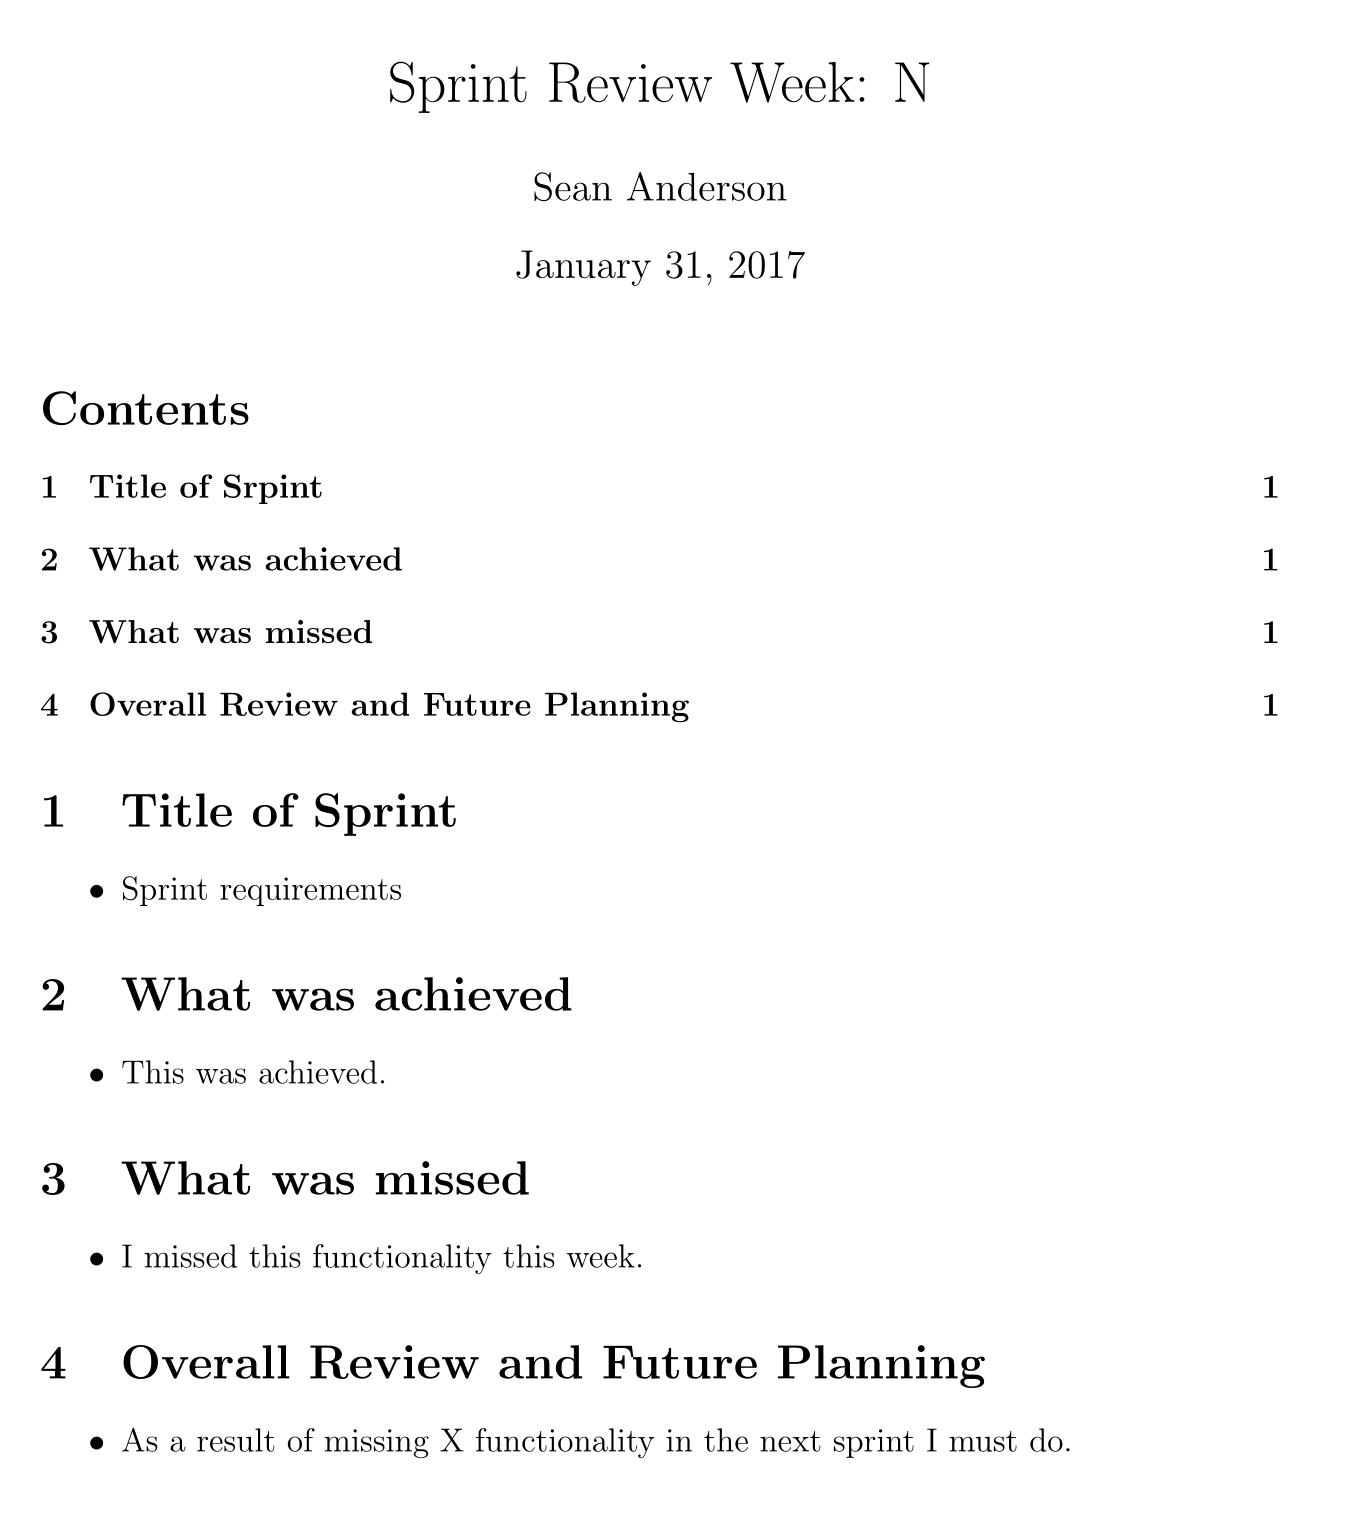
\includegraphics[width=\textwidth,height=\textheight,keepaspectratio]{images/sr}
\caption{The Sprint review template}
\end{figure}

\subsection{Initial Requirements}
Before splitting the different tasks into stories, it is important to consider the overall requirements of the system. Anybody must be able to register for an account; there will be three different types of account (a general music lover, an artist and a venue owner.) The general music lover should be able to follow artists and view events which are relevant to them. An artist should have the same functionality of a music lover however they will appear in a different section of the app. This is so it makes it easier for people to know who they are following. Both artists and music lovers should be able to post and people who follow them will see this post.

Venue owners need to be able to create events and add artists to these events. Music lovers should then be able to see all of the appropriate information about these events. In terms of suggesting to the user who they should follow and what events they should attend, there will be some machine learning code placed on the back end of the system. As well as this the app will need to be styled.

\subsection{Stories}
As Scrum is an agile methodology the project was split into multiple different stories. These include:
\begin{itemize}
	\item A register system so that all user types can create an account.
	\item A follow system so that users can follow other users.
	\item A post system so that when a user posts, all people who follow them can see that post.
	\item A create events system which can only be used by venue owners.
	\item Styling of the app.
	\item Machine learning code on the back end of the system which will mean users will get appropriate suggestions.
\end{itemize}

\subsection{Framework}
There are multiple different frameworks for developing apps using hybrid technologies. These frameworks all use web technologies however it differs from framework to framework as to what specific web technology is used. For example apps made using the JQuery Mobile Framework are wrote in JQuery and apps made using the ionic framework are written in AngularJS.

As well as considering the language of the framework it was also important to consider other factors before deciding which framework would be most appropriate. These factors include things such as page change speed, access to native APIs and external documentation and community available for support.

The below table summarises information about multiple different hybrid app frameworks.

//TODO make table here.

Despite Ionic having a steep learning curve due to it using AngularJS as opposed to JQuery it seemed like the most appropriate framework to use. This is because not only does Ionic have a fairly substantial amount of middleware plugins which will allow for platform specific APIs to be accessed but it is also considered one of the fastest frameworks, so this will aid the project aim of discovering whether hybrid apps are feasible alternatives to native apps. 

